\documentclass{article}

\usepackage{fancyhdr}
\usepackage{extramarks}
\usepackage{amsmath}
\usepackage{amsthm}
\usepackage{amsfonts}
\usepackage{tikz}
\usepackage[plain]{algorithm}
\usepackage{algpseudocode}
\usepackage{enumerate}
\usepackage{amsmath}
\usepackage{amssymb}
\usetikzlibrary{automata,positioning}

%
% Basic Document Settings
%

\topmargin=-0.45in
\evensidemargin=0in
\oddsidemargin=0in
\textwidth=6.5in
\textheight=9.0in
\headsep=0.25in

\linespread{1.1}

\pagestyle{fancy}
\lhead{\hmwkAuthorName}
\chead{\hmwkClass\ (\hmwkClassInstructor\ \hmwkClassTime): \hmwkTitle}
\rhead{\firstxmark}
\lfoot{\lastxmark}
\cfoot{\thepage}

\renewcommand\headrulewidth{0.4pt}
\renewcommand\footrulewidth{0.4pt}

\setlength\parindent{0pt}

%
% Create Problem Sections
%

\newcommand{\enterProblemHeader}[1]{
    \nobreak\extramarks{}{Problem \arabic{#1} continued on next page\ldots}\nobreak{}
    \nobreak\extramarks{Problem \arabic{#1} (continued)}{Problem \arabic{#1} continued on next page\ldots}\nobreak{}
}

\newcommand{\exitProblemHeader}[1]{
    \nobreak\extramarks{Problem \arabic{#1} (continued)}{Problem \arabic{#1} continued on next page\ldots}\nobreak{}
    \stepcounter{#1}
    \nobreak\extramarks{Problem \arabic{#1}}{}\nobreak{}
}

\setcounter{secnumdepth}{0}
\newcounter{partCounter}
\newcounter{homeworkProblemCounter}
\setcounter{homeworkProblemCounter}{1}
\nobreak\extramarks{Problem \arabic{homeworkProblemCounter}}{}\nobreak{}

%
% Homework Problem Environment
%
% This environment takes an optional argument. When given, it will adjust the
% problem counter. This is useful for when the problems given for your
% assignment aren't sequential. See the last 3 problems of this template for an
% example.
%
\newenvironment{homeworkProblem}[1][-1]{
    \ifnum#1>0
        \setcounter{homeworkProblemCounter}{#1}
    \fi
    \section{Problem \arabic{homeworkProblemCounter}}
    \setcounter{partCounter}{1}
    \enterProblemHeader{homeworkProblemCounter}
}{
    \exitProblemHeader{homeworkProblemCounter}
}

%
% Homework Details
%   - Title
%   - Due date
%   - Class
%   - Section/Time
%   - Instructor
%   - Author
%

\newcommand{\hmwkTitle}{Tutorial Week 8}
\newcommand{\hmwkDueDate}{March 4, 2021}
\newcommand{\hmwkClass}{CZ4041}
\newcommand{\hmwkClassTime}{CS4}
\newcommand{\hmwkClassInstructor}{Assoc Prof Pan, Sinno Jialin}
\newcommand{\hmwkAuthorName}{\textbf{Pang Yu Shao}}
\newcommand{\hmwkAuthorID}{\textbf{U1721680D}}

%
% Title Page
%

\title{
    \vspace{2in}
    \textmd{\textbf{\hmwkClass:\ \hmwkTitle}}\\
    \normalsize\vspace{0.1in}\small{Due\ on\ \hmwkDueDate\ at 8:30am}\\
    \vspace{0.1in}\large{\textit{\hmwkClassInstructor\ - \hmwkClassTime}}
    \vspace{3in}\\
    \hmwkAuthorName\\
    \hmwkAuthorID
}

\date{04/03/2021}

\renewcommand{\part}[1]{\textbf{\large Part \Alph{partCounter}}\stepcounter{partCounter}\\}

%
% Various Helper Commands
%

% Useful for algorithms
\newcommand{\alg}[1]{\textsc{\bfseries \footnotesize #1}}

% For derivatives
\newcommand{\deriv}[1]{\frac{\mathrm{d}}{\mathrm{d}x} (#1)}

% For partial derivatives
\newcommand{\pderiv}[2]{\frac{\partial}{\partial #1} (#2)}

% Integral dx
\newcommand{\dx}{\mathrm{d}x}

% Alias for the Solution section header
\newcommand{\solution}{\textbf{\large Solution}}

% Probability commands: Expectation, Variance, Covariance, Bias
\newcommand{\E}{\mathrm{E}}
\newcommand{\Var}{\mathrm{Var}}
\newcommand{\Cov}{\mathrm{Cov}}
\newcommand{\Bias}{\mathrm{Bias}}

\begin{document}

\maketitle

\pagebreak

\begin{homeworkProblem}
    Consider a 2-dimensional dataset for two-class classification by SVM, as shown in Figure 1, where the 
    red "square" and the blue "circle" denote the positive and negative classes respectively. Is this 
    dataset seperable by a linear SVM classifier? If no, why? If yes, what is the decision boundary of the 
    linear SVM? And what are the pair of parallel hyperplanes associated with the decision boundary? (No need to provide proofs) 
    \begin{figure}[H]
        \begin{center}
        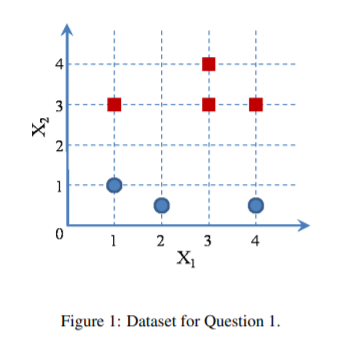
\includegraphics{resources/q1.PNG}
        \end{center}
    \end{figure}


    \textbf{Solution}\\
    Decision boundary: $X_2 = 2$\\\\

    Pair of parallel hyperplanes: $X_2 = 1$ and $X_2 = 3$
\end{homeworkProblem}
\newpage
\begin{homeworkProblem}
    Please induce why the two parallel hyperplane of a decision boundary.
    \begin{center}
        $\mathbf{w}\cdot\mathbf{x} + b = 0$
    \end{center}
    can be written as\\
    \begin{center}
        $\mathbf{w}\cdot\mathbf{x} + b = k$, and $\mathbf{w}\cdot\mathbf{x} + b = -k$
    \end{center}
    where $k > 0$, respectively as shown on the 18th Slide of the lecture notes "Lecture 8a"\\\\
    \textbf{Solution}\\
    Let $x_1$ and $x_2$ be points on the two parallel hyperplanes, and $x_0$ be a point on the 
    decision boundary that is between $x_1$ and $x_2$.\\\\

    $b_{11}: \mathbf{w}\cdot\mathbf{x_1}+b = k$, where $k > 0$\\
    $b_{12}: \mathbf{w}\cdot\mathbf{x_2}+b = k'$, where $k' < 0$\\
    $B_1: \mathbf{w}\cdot\mathbf{x_0}+b = 0'$\\\\

    $\mathbf{w}\cdot\mathbf{x_1}+b = k$\\
    $\mathbf{w}\cdot\mathbf{x_0}+b = 0$\\\\
    $\mathbf{w}\cdot\mathbf{x_1} = k - b$\\
    $\mathbf{w}\cdot\mathbf{x_0} = -b$\\\\
    $\mathbf{w}\cdot\mathbf{(x_1-x_0)} = k$\\
    $\mathbf{||w||_2}\times\mathbf{||x_1-x_0||_2}\times cos(0) = k$\\
    $\mathbf{||w||_2}\times\mathbf{||x_1-x_0||_2} = k$\\\\

    Similarly,\\
    $\mathbf{||w||_2}\times\mathbf{||x_2-x_0||_2}\times cos(180) = k'$\\
    $\mathbf{||w||_2}\times\mathbf{||x_2-x_0||_2} = -k'$\\\\

    Since $||x_1-x_0||_2 = ||x_2-x_0||_2$,\\
    $k = -k'$, or $k' = -k$\\\\

    Therefore, the two parallel hyperplanes can be written as  $\mathbf{w}\cdot\mathbf{x} + b = k$, 
    and $\mathbf{w}\cdot\mathbf{x} + b = -k$

\end{homeworkProblem}



\end{document}